
\section{Introduction}
A vector predictor can approximate an intervention's internal response yet mispredict its downstream effect. We ask whether a subspace fitted from native vector responses, without direct readout labels, identifies a repairable component of that error, and how far such a diagnosis transfers. The question is empirical: reducing vector error need not reduce readout error, even for a linear readout.

Historical experiment E041 found an unusually concentrated benefit on Qwen3-0.6B-Base: oracle correction in a rank-eight response space reduced is/are readout MSE by 98.85\%, versus 14.44\% in its complement. The original forecast had favored outside repair, so this was exploratory. We now test the same frozen predictor, subspace, layer-21 target and upstream-neuron intervention on 64 fresh lexical blocks. Inside repair reduces MSE by 99.25\%; outside by 8.38\%. The result is no longer supported only by the historical sample.

A separate three-fit study asks whether the benefit distinguishes FIT-derived spaces from simple alternatives. At rank eight, oracle projection reduces mean loss by 88.13\%, versus 1.18\% for the fixed same-rank random spaces and 5.30\% for random corrections rescaled to the FIT correction norm. These controls concern the new predictors, not a direct randomized comparison of the historical predictor. All six ranks are retained; rank 32 improves further. Thus FIT-derived spaces identify an oracle-correctable error component in this setting; the result does not identify a uniquely special dimension eight.

The other studies establish limits. In Qwen's separate layer-27 aligned study, the same three fitted pairs help on T2 but harm on T5. Gemma-270M benefits on both frames; separate Gemma-1B and Llama-1B cohorts establish T5 harm; Llama benefits on T2. A failed ranking prediction and fitted-object substitutions constrain transfer. Finally, accurate oracle sign prediction does not imply useful learned repair: a gate worsens the original predictor on Qwen T5, and a direct ridge map trained on the same 256 available vector labels has lower loss on both frames. In contrast, a new prospective L21 test now establishes useful learned correction relative to the historical predictor, while full-vector direct prediction has lower mean loss.

The new L21 learned study reuses 384 existing FIT vector labels and freezes its models before another 64-block TEST. A rank-eight residual correction reduces readout MSE by 97.21\%, but Direct384 has 23.97\% lower mean loss than correction (equivalently, correction has 31.52\% higher loss). A direct refit restricted to the same $U$ span also has slightly lower point loss. The contribution is this controlled chain: replicated oracle repairability, separate rank/norm controls, measured learned utility against strong baselines, and context/fitted-object limits. Table~\ref{tab:scope} separates the cohorts and inferential status. Four checkpoints appear, but the oracle and learned384 L21 tests use one checkpoint and one readout; they are not four-model confirmation of low-dimensional repair.
\begin{table}[ht]
\centering\scriptsize\setlength{\tabcolsep}{4pt}
\begin{tabular}{>{\raggedright\arraybackslash}p{.15\textwidth}>{\raggedright\arraybackslash}p{.25\textwidth}>{\raggedright\arraybackslash}p{.25\textwidth}>{\raggedright\arraybackslash}p{.25\textwidth}}
\toprule Claim/study & Cohort and reuse & Frozen before which outcomes? & Reporting status and result\\\midrule
E041 motivation & Qwen-0.6B L21; primary B5/F1; whole MAIN 16 blocks & Original forecast favored outside repair; observed inside benefit motivates later work & Historical result, not retroactive confirmation: 98.85\% inside versus 14.44\% outside MSE reduction.\\[3pt]
Fresh E041 replication & Qwen-0.6B L21; 64 new blocks, original B5/F1 & Historical fit/operator, cohort and analysis fixed before TEST; all forecasts frozen before targets & Independent completion approved; nominal block intervals. Inside/outside reductions 99.25\%/8.38\%.\\[3pt]
Rank controls & Same 64 TEST blocks; three separate new FIT cohorts & Six ranks and random seeds fixed; vector labels only select spaces & Conditional on three fits; rank8 reduction 88.13\%, versus 1.18\% random and 5.30\% norm-rescaled.\\[3pt]
Learned L21 & Another 64 fresh TEST blocks; reuses the 24 FIT blocks (384 labels) & FIT-only selection and all predictions frozen before new TEST targets & Nominal fixed-fit block intervals; C improves P by 97.21\%, but loses to Direct384.\\[3pt]
Budget readout & Third distinct 64-block L21 TEST; one FIT0/seed17 sequence, 32--384 labels & All forecasts frozen before fresh targets; 384 uses full pool & Fixed-fit nominal interval favors C32; Direct has lower mean at 64--384.\\[3pt]
New FIT32/readout & Same budget TEST reused posthoc; six new FIT blocks in three two-block cohorts & Vector-only fits and forecasts frozen before new suffix calls; TEST already exposed & Conditional nominal intervals; mixed per-fit rankings; have/has mean favors Direct, is/are interval crosses zero.\\[3pt]
Aligned repair & Qwen-0.6B L27 and Gemma-270M L17; same 256 new blocks; three fixed fits/model & Fits, T5 primary contrast and analysis fixed before finite repair outcomes & Nominal pointwise 95\% intervals; T2/outside descriptive. Gemma helps both; Qwen helps T2, harms T5.\\[3pt]
Earlier confirmation & Gemma-1B/Llama-1B, separate 256-block cohorts; one fit/model & Their original contrasts/families fixed before TEST & Original family decisions retained: T5 harm in both; Gemma ranking reversal fails.\\[3pt]
Fitted-object diagnosis & Gemma-1B cached states; historical 32/current 256-block cohorts & Crosses chosen after the ranking changed & Posthoc fixed-state substitutions: mean ranking follows subspace-pair version; no causal training-domain claim.\\[3pt]
Forecast/utility & Qwen aligned 256; supporting 32-block study on Gemma-1B, Llama-1B, Gemma-270M & Forecast/correction recipes sealed before finite repair readouts; Gemma-1B cached extension retrospective & Descriptive dependent-cell accuracies; oracle signs accurate, learned gate loses to the better always/never policy in every supporting scope. No pooling with aligned $N$.\\
\bottomrule
\end{tabular}
\caption{Claim and inference map. Rows are successive questions, not interchangeable replications. The 32-block scopes use three fixed fits/model and mixed acquisition timing; details remain in the appendices.}\label{tab:scope}
\end{table}
The subsequent budget and new-FIT/readout studies sharpen that conclusion. A fixed 32-label C predictor beats Direct32 on fresh is/are TEST, whereas Direct has lower mean loss at every larger tested budget. Three disjoint new FIT32 cohorts then yield mixed rankings on the reused TEST: the new have/has readout favors Direct on average, and the is/are interval crosses zero. The benefit is observed in one fixed training sequence; the later three fits give mixed rankings and do not establish stable superiority across FIT draws or readouts. Historical priors consume additional resources beyond the stated new-label budget.

\section{Relation to existing work}
The closest precedent is the decomposition and partial repair of sparse-autoencoder error by Engels et al.~\cite{engels2024}. That work studies natural-activation reconstruction error and downstream cross-entropy. Here the target is a \emph{native intervention delta}: a vector predictor approximates a donor-induced branch response, and the outcome is squared error in its predicted is/are logit-margin effect. E041's space is selected from vector responses without direct readout labels; the fresh L21 replication and separate rank/norm controls test that concrete concentration, while subsequent studies connect repair effects to fitted-object substitutions and learned correction baselines. This difference specifies the empirical question, not a claim of methodological superiority.

Subspace activation patching already has documented interpretability pitfalls~\cite{makelov2023}; self-repair gives relevant context for compensating internal changes~\cite{rushing2024}. Counterfactual response subspaces and geometry adaptation are also established topics~\cite{tang2026,lim2026}. Gradient-aware sparsification and native computational-graph methods precede this study~\cite{farnik2025,ameisen2025}. We therefore claim neither projection repair nor Taylor/Jacobian forecasting as a new method. The contribution is the specific controlled empirical chain summarized in Table~\ref{tab:scope}, bounded to the reviewed literature rather than an assertion of worldwide priority.
\section{Prediction and oracle repair}
For a fixed recipient and intervention $I$, let $D=y_I-y_0$ be the native target-branch output change. Direct donor-input patching gives $D=M(x_d)-M(x)$; the L21 study instead measures the response to upstream neuron edits. Let $g_I(v)$ be the final logit margin after inserting $y_0+v$ at the target and running its actual native suffix. The upstream state is held fixed within each comparison: the L21 tests retain the residual produced by $I$, whereas the direct-patch studies retain the recipient residual. Write $g=g_I$ below; use the same reference $g(0)$ for native and predicted effects. Set
\[
 H=g(D)-g(0),\qquad h(v)=g(v)-g(0),\qquad L(v)=[H-h(v)]^2.
\]
A ridge map predicts $P$ from target-free input changes (the L21 B5 map uses layer-20/21 changes; direct-patch studies use $x_d-x$). An orthonormal matrix $U\in\mathbb R^{d\times r}$ is fitted from native vector responses without direct is/are labels; $r=8$ unless the rank sweep is specified. The oracle inside and complement repairs are
\[
 P_U=P+UU^\top(D-P),\qquad P_{out}=D-UU^\top(D-P).
\]
Both use the true TEST delta $D$ and are diagnostics, not deployable learned corrections. Inside repair reduces squared vector error by $\|UU^\top(D-P)\|^2$; outside removes $\|(I-UU^\top)(D-P)\|^2$. Full oracle $D$ has zero readout-prediction error by definition, not as an independent technical correctness control. That algebra does not determine downstream loss. Writing $e=H-h(P)$ and $a=h(P_U)-h(P)$ gives
\[
 L(P_U)-L(P)=a^2-2ea.
\]
The identity organizes the measured effects; it is not itself a new mechanism or discovery. A positive loss contrast denotes worse prediction of the intervention's readout effect, not poorer natural grammatical accuracy.

\section{Experimental design}
\subsection{Fresh L21 replication and separate rank controls}\label{sec:l21design}
The replication preserves E041's Qwen3-0.6B-Base checkpoint, historical B5 predictor and rank-eight $U$, target layer 21 and F1 prompt, ``The \{subject\} that the \{attractor\} can see''. It uses 64 fresh unordered lexical pairs, each in four subject/attractor-number forms. Donors reverse subject number. At the final position, the native layer-19 SwiGLU coordinate 1317 is moved toward its donor value with dose $c\in\{.5,1\}$. Branch B leaves layer 20 free; branch C restores recipient layer-20 coordinate 1423. Thus each block supplies 16 conditions, giving 1,024 conditions. Layer indices are zero-based. The response $D$ is the resulting layer-21 output difference, not a donor-input patch at layer 21.

B5 predicts from the measured target-free layer-20 and layer-21 input changes,
\[
 P=\operatorname{FP32}\!\left([\Delta x_{20}/s_{20},\Delta x_{21}/s_{21}]W U^\top/\sqrt2\right).
\]
The historical $s,W,U$ are unchanged. Patches retain the actual upstream-intervention residual and propagate through native layers 22--27, final norm and readout. E041's readout is logit(\texttt{ are}) minus logit(\texttt{ is}); reversing both native and predicted margins in the other studies leaves MSE unchanged. FP32 native arithmetic and FP64 fitting/projection follow the historical path, with independently qualified suffix batching. No CLT is involved.

The separate rank study fits three new predictors on disjoint groups of eight lexical blocks each (128 native vector labels/group). Each uses the same B5 input construction, fixed $\lambda=10^{-4}$ and an eight-dimensional prediction factorization. Uncentered SVD of that group's native FIT deltas supplies nested response spaces at ranks 1, 2, 4, 8, 16 and 32. Fixed Gaussian-QR draws supply same-rank random spaces. For each new predictor and rank, we compare exact oracle projection into the FIT-derived or random space, and a distinct random correction rescaled to the FIT-derived correction norm. This last arm is not an orthogonal projection. Seeds, ranks and operators were fixed before TEST; no readout labels select $U$ and no rank is selected from the outcomes.

The three fits share the same 64 TEST blocks. We average conditions and, for rank summaries, fits within each block; $N=64$, not 192 or 3,072. All TEST input captures and predictions were frozen before any TEST target. Freshness is relative to the recorded local exposure inventory, not pretraining. The primary historical-fit report is the equal-block MSE contrast across both branches and doses. Saved nominal 95\% paired block intervals use 1,999 draws, seed 3110301; they condition on the fixed fits and do not claim familywise error control or fit-population power. The new-fit rank study is not a refit of the historical predictor, and must not be conflated with the learned experiment below.

\subsection{Prospective learned correction at L21}\label{sec:learneddesign}
We preserve the historical $P,U$, scale factors, layer and upstream operator, but use another 64 fresh lexical pairs (256 prompts, 1,024 conditions), disjoint from both the preceding 64-block TEST and the recorded exposure inventory. The 384 native vector labels from the three preceding FIT groups are reused for training; no previous TEST targets select the models. Let $\phi=[\Delta x_{20}/s_{20},\Delta x_{21}/s_{21}]/\sqrt2$ and train a coefficient predictor $\widehat a(\phi)$ on $U^\top(D-P)$. The learned correction is
\[
 C=P+U\widehat a(\phi).
\]
The features require native upstream target-free prefixes, but not the layer-21 output delta $D$ being predicted. All 1,024 predictions are frozen before the first native TEST target. Model selection uses vector/coefficient losses only: three outer held-out FIT groups diagnose prediction, and four-fold block CV selects final models on all 24 FIT blocks. Linear/RBF ridge candidates are allowed for C and Direct384; the same-$U$ comparator is a linear direct predictor restricted to the historical span. The final models all select linear ridge with $\lambda=10^{-6}$ and use all 384 labels, with no TEST tuning. This is the lower boundary of the frozen grid, not evidence of an interior optimum; smaller penalties were not tested.

We compare seven arms: historical $P$, $C$, same-$U$ direct refit, full-vector Direct384, $P$ plus mean FIT coefficient correction, oracle inside repair, and zero-change. The oracle arm uses true TEST $D$ and is diagnostic. Zero-change predicts the original natural margin; under the changed upstream residual it is not generally equivalent to inserting a zero target-layer delta. All other predicted vectors use the actual intervened residual and native nonlinear suffix. Equal additional label budgets do not equalize total training information: historical $P,U$ and scales carry earlier fitting information.

The primary contrast is $L(C)-L(P)$; $L(C)-L(\mathrm{Direct384})$ is secondary. We average the 16 conditions within each of 64 blocks. Nominal paired 95\% intervals use the frozen 1,999-draw block bootstrap, conditional on the fixed fits. Other arms and branch/dose/number subgroups remain descriptive. The earlier oracle TEST and this learned TEST are separate cohorts, not pooled replication units.

\subsection{C is prior-centered kernel ridge}\label{sec:priorridge}
All three predictors use the same linear-in-target ridge smoother, with different targets and decoding. In row notation let $X$ contain the normalized inputs, $Y=DU$, and $P\simeq XWU^\top$, with orthonormal $U$. Training centers $X$ and each target; prediction adds its training target mean. For $A=X-\bar X$, the smoother is
\[
 F(Y)(x)=\bar Y+k(x)(K+n\lambda I)^{-1}(Y-\bar Y).
\]
For the linear kernel $K=AA^\top$; for RBF, $K_{ij}=\exp(-\|a_i-a_j\|^2/s)$, where $s$ is the median positive training squared distance. No width search or further feature standardization is performed. The frozen penalty grid is $\{1,10^{-2},10^{-4},10^{-6}\}$. C and Direct search both kernels; same-$U$ searches only the four linear candidates in learned384 and the original budget study. The later three-FIT32 study searches all eight candidates for every method. Selection is separate by method and uses vector losses, not readout labels.

Ignoring FP32 projection rounding, C predicts $(xW+F(Y-XW)(x))U^\top$, same-$U$ predicts $F(Y)(x)U^\top$, and Direct predicts $F(D)(x)$. For the linear kernel C is exactly ridge around the historical coefficient map:
\[
 \Gamma_C=\arg\min_\Gamma\{\|Y_c-A\Gamma\|_F^2+n\lambda\|\Gamma-W\|_F^2\},
 \qquad \widehat Y_C(x)=\bar Y+(x-\bar X)\Gamma_C.
\]
This identity requires the same inputs, centering, unpenalized intercept and $n\lambda$ convention, and $P=XWU^\top$ in exact arithmetic. The implementation rounds P to FP32, so its exact target is $(D-P)U$ and the algebra has that numerical qualification. Same-$U$ instead shrinks toward zero. For RBF, C is a kernel-ridge residual predictor around mean function $xW+\overline{Y-XW}$; its formula has the familiar GP posterior-mean form conditional on that chosen mean and noise parameter \cite{rasmussen2006}. No GP uncertainty estimate or probabilistic calibration is implemented. Prior-centered regression and mean-function residual fitting are established methods, not a new algorithm here.

With a common fixed smoother, $F(DU)=F(D)U$ exactly: same-$U$ is Direct projected back into $U$. C differs from it by $P-F(PU)U^\top$ (up to rounding). Positive ridge penalties need not reproduce the prior, and separately selected kernels or penalties invalidate a common-smoother identity. At 384 labels all three saved models choose linear/$10^{-6}$; saved same-$U$ and projected-Direct coefficient weights agree within $1.69\times10^{-11}$. This does not imply identical full-vector predictions. The prior's historical information is additional to the new-label budget. The full-vector residual comparator $P+F(D-P)$ would separate prior use from the output-span restriction, but is not a completed approved result in this manuscript.


\subsection{Aligned L27/L17 comparison}
The separate aligned comparison uses Qwen3-0.6B-Base and Gemma-3-270M on the same 256 new lexical blocks, two held-out syntactic frames and four subject/distractor conditions per frame: 2048 documents per model. T2 is ``Near the enclosure, the \{s\} that the \{a\} can observe''; T5 is ``Everyone agrees that the \{s\}, unlike the \{a\},''. Donors reverse subject number within a block, frame and distractor condition. The readout is logit(\texttt{ is}) minus logit(\texttt{ are}), including the leading spaces. Lexical freshness is relative to the recorded local exposure audit, not pretraining.

The tested branch is at the final prompt position in the final block: layer 27 for Qwen and layer 17 for Gemma. Qwen uses its raw SwiGLU output; Gemma includes post-feedforward normalization. The recipient residual stays fixed, and the actual final norm and output head determine the readout. Native/head arithmetic is FP32; vector fitting and projection are FP64. These L27/L17 experiments change the intervention and fitting recipe relative to E041. They remain distinct from the fresh L21 replication above; their sign differences do not isolate layer as a causal factor.

Each model has three fixed matched predictor/subspace pairs. A centered ridge map ($\lambda=.01$) predicts the native delta from the donor-minus-recipient input; a separate response sample supplies the leading eight right singular vectors for $U$. Each pair uses 128 FIT\_MAP and 128 FIT\_U documents. Fitting frames F0/F1 differ from TEST frames T2/T5. Gemma reuses three accepted fits; Qwen uses three new disjoint FIT groups. No direct is/are labels select $U$. Technical parity checks precede the tests. Appendix~\ref{sec:methods} gives the fitting equation, checkpoint identity and earlier-study designs.

We average the three fits and four conditions \emph{within each lexical block} before inference. The independent sampling unit is therefore the block ($N=256$), not a condition or fit-by-condition cell. Primary T5 inside-minus-predictor loss was fixed before outcomes; T2 and inside/outside comparisons are descriptive. Saved nominal pointwise 95\% intervals use 1999 block draws and fixed seeds. They do not inherit the calibrated 99\% decision families of the earlier single-fit studies, and no fit-population uncertainty or new power assurance is claimed. All manuscript numbers reproduce saved summaries; manuscript preparation performs no refitting, model calls or resampling.
\subsection{Shared data and distinct estimands in the companion study}
The companion manuscript, \emph{A Dose-Dependent Crossover in Transcoder Fidelity: Held-Out Prediction and Residual Geometry}, studies a different estimand using some of the same Qwen data (Table~\ref{tab:shared}). It adopts the unit-dose native and first-fit ridge outputs and adds public-CLT dose-response measurements; this paper evaluates oracle and learned repair of vector predictions. These analyses are not independent replications. The companion is identified by its current title; no public identifier or authorship is asserted before release.
\begin{table}[ht]\centering\scriptsize\setlength{\tabcolsep}{4pt}
\begin{tabular}{>{\raggedright\arraybackslash}p{.16\textwidth}>{\raggedright\arraybackslash}p{.35\textwidth}>{\raggedright\arraybackslash}p{.39\textwidth}}
\toprule Scope & Shared foundation / separation & Unique measurements and estimand\\\midrule
Qwen-0.6B A/B & Same Base checkpoint, L27/is--are, 256 T2/T5 blocks and 2048 contexts, donor pairs and captured $x,R,y$. B reuses r1 FIT\_MAP 128, $P_{r1}$ and 2048 native +2048 $P_{r1}$ unit-dose margins. & A: three P/U pairs, inside/outside oracle, forecasts and learned repair/gate, full residual and Direct256. B: public CLT/FROZEN/Taylor and six doses, with dose-specific r1 ridge/mean. The 4096 reused margins are not Direct256 outputs.\\[3pt]
Qwen-0.6B L21 A & Three distinct 64-block F1 TEST cohorts and 24 reused FIT blocks, plus six new FIT blocks in the later study; upstream neuron intervention, target L21. No shared B dose-response cohort. & First TEST: original-fit oracle replication and rank controls. Second TEST: learned correction and Direct384. Third TEST: budgets; subsequently reused posthoc for three new FIT32 cohorts and have/has readout. FIT totals are 24 reused plus six new blocks, not extra independent TEST replications.\\[3pt]
Gemma-270M A & Agreement T2/T5, 2048 contexts, L17/is--are, three P/U pairs. & Oracle/learned repair; final transformer block. These are not B's native captures.\\[3pt]
Gemma-270M B & Separate name-pair corpus, 1536 contexts, so/when/transfer, L15/she--he; separate FIT/PILOT and public TC. & Dose fidelity through native L16/17. Its posthoc cache/geometry studies reuse B rather than add independent blocks.\\
\bottomrule\end{tabular}
\caption{Cross-manuscript data provenance. Reuse avoids duplicate measurement; it does not increase independent sample size. FIT128 and the distinct Direct256 comparator must not be conflated.}\label{tab:shared}
\end{table}

\section{Repair is effective but conditional}
\subsection{Fresh replication of the low-dimensional benefit}\label{sec:l21results}
Historical E041's primary B5/F1 contrast gave 98.85\% inside and 14.44\% outside MSE reduction on a 16-block MAIN cohort. Its original forecast favored outside repair, so the inside benefit was exploratory. The fresh test preserves the selected fit and operator rather than retrospectively changing that history. Table~\ref{tab:l21} now shows a 99.25\% inside reduction on 64 new lexical blocks. The paired inside-minus-B5 loss is $-.0144172$, with nominal 95\% interval $[-.0160698,-.0129072]$. The reduction is 99.07--99.30\% across all four branch/dose subgroups. Outside improves by 8.38\%, not the historical 14.44\%.

\begin{table}[ht]\centering\small
\begin{tabular}{lrrr}\toprule
Frozen historical fit & Readout MSE & Reduction vs. B5 & Paired loss change\\\midrule
B5 prediction & .01452685 & --- & ---\\
Oracle inside, rank 8 & .00010961 & 99.245\% & $-.01441724$\\
Oracle outside & .01330943 & 8.381\% & $-.00121742$\\
Full oracle & $1.31\times10^{-11}$ & numerical floor & ---\\
\bottomrule\end{tabular}
\caption{Fresh E041/L21 replication: 64 blocks, 1,024 conditions, original frozen B5/$U$. Inside and outside have unequal dimension/norm budgets. Full-oracle residual error reflects FP32 patch/suffix arithmetic; it is not an independent scientific result.}\label{tab:l21}
\end{table}

This confirms a specific empirical concentration: a space chosen from vector FIT responses without direct readout supervision captures a component whose oracle correction almost eliminates this readout error on fresh pairs. It does not show that eight coordinates explain the model, nor that the two reduction percentages are additive contributions to a mechanism.

\subsection{Separate fits distinguish response structure from random controls}
The three new FIT predictors have equal-fit mean baseline MSE $.00075285$, different from historical B5. At rank eight, oracle repair in their own FIT-derived spaces gives MSE $.00008939$ (88.13\% reduction), compared with $.00074397$ (1.18\%) for the fixed random spaces of equal rank and $.00071299$ (5.30\%) for the norm-rescaled random corrections. Figure~\ref{fig:ranks} retains all six ranks. FIT-derived spaces have lower mean loss than these controls at every rank. Their rank-eight paired change relative to their own baselines is $-.00066347$; its saved nominal 95\% interval is $[-.00081751,-.00052898]$, conditional on these three fits. No additional pairwise significance family is introduced.

\begin{figure}[ht]\centering
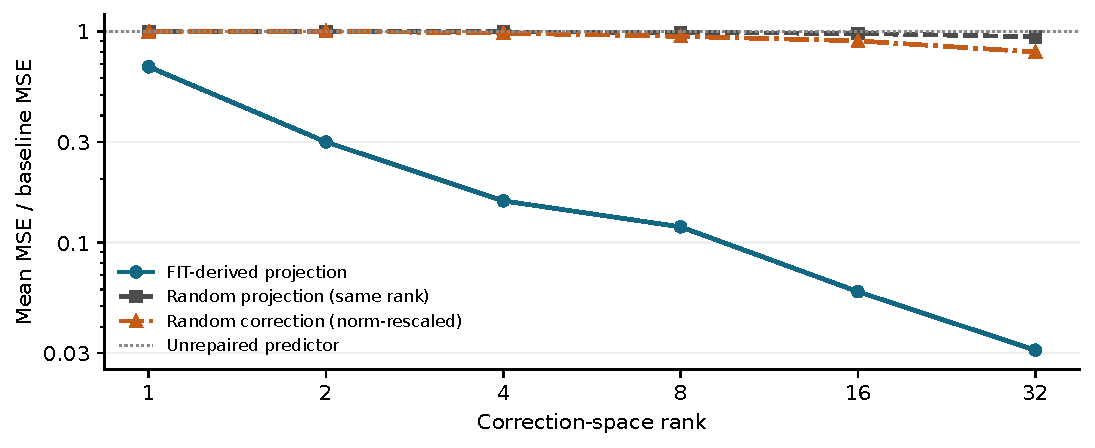
\includegraphics[width=.88\textwidth]{l21_rank_controls.pdf}
\caption{Separate new-fit L21 study: equal-fit mean MSE on the same 64 TEST blocks, normalized by the common equal-fit baseline for display. All points derive from accepted summaries without refitting or resampling. Random and FIT-derived exact projections have the same rank; the random norm-rescaled arm additionally matches correction magnitude and is a distinct intervention. Fixed random draws are controls, not a distribution over all random spaces.}\label{fig:ranks}
\end{figure}

The FIT-space reductions at ranks 1/2/4/8/16/32 are 32.01/70.06/84.24/88.13/94.14/96.90\%. Thus eight dimensions are effective, but not uniquely optimal. At small ranks the random-control changes are tiny or uncertain; for example, the nominal paired interval for rank-one random repair includes zero. The norm-matched controls address correction magnitude in this new-fit study, but must not be presented as a randomized comparison for the unchanged historical B5. These two oracle studies are followed by the separate prospective learned test below.
\subsection{Learned L21 correction helps; direct prediction has lower mean loss}\label{sec:learnedresults}

On the separate 64-block prospective TEST, C reduces historical P readout MSE by 97.21\% (Table~\ref{tab:learnedL21}). Its paired primary loss change is $-.0149633$, with nominal 95\% interval $[-.01669,-.01329]$. This is measured downstream utility without true TEST-error access, not the FIT-only coefficient prediction score.

\begin{table}[ht]\centering\small

\begin{tabular}{lrrr}\toprule Arm & Readout MSE & Vector squared error & Coefficient squared error\\\midrule

Historical P & 0.01539272 & 4.08662 & 1.24271\\

Learned C & 0.00042944 & 2.89175 & 0.04785\\

Same-$U$ direct & 0.00040599 & 2.88978 & 0.04587\\

Direct384 & 0.00032652 & 0.29801 & 0.04587\\

Mean correction & 0.01605005 & 4.07251 & 1.22861\\

Oracle inside & 0.00008828 & 2.84390 & 0.00000\\

Zero-change & 0.76689144 & 5.93717 & 3.09327\\

\bottomrule\end{tabular}

\caption{New learned L21 TEST: 64 blocks, 1,024 conditions, frozen models trained with 384 reused FIT labels. Vector columns are mean squared L2 errors, not relative errors. Oracle is diagnostic. Zero-change uses the original natural margin.}\label{tab:learnedL21}

\end{table}

Direct384 has lower mean MSE than C: the secondary C-minus-Direct384 contrast is $+.000102919$, nominal 95\% interval $[+.000036397,+.000174289]$. C therefore has 31.52\% higher loss than Direct384. The same-$U$ linear direct predictor also has lower point loss than C, although this is not an additional corrected hypothesis test. A mean coefficient correction increases loss by $.000657337$ relative to P. The gain is not reproduced by the tested FIT-mean correction.


Relative to Direct384, C has about 9.7 times the mean squared vector error but only 31.52\% higher readout MSE. This descriptive comparison shows that the two losses weight prediction errors differently in this fixed setting; it does not identify which error directions cause the difference or establish transfer to another readout.

C improves P in all reported branch/dose/subject/attractor marginal groups. Direct384 has lower mean loss in both branches and doses, but the descriptive S=1 subgroup slightly favors C; no subgroup is selected or tuned after TEST. The full subgroup table remains in the saved summary. Oracle inside again has substantially lower loss, but neither its value nor the earlier 99.25\% reduction is treated as a learned-method guarantee.

The earlier FIT-only outer evaluation reduced coefficient squared error by about 95.8\%; that metric did not establish readout improvement. The new TEST supplies that missing measurement. Nevertheless, direct prediction remains stronger overall. Learning residual coefficients under a historical prior is therefore useful here without being a superior new learning method.

\subsection{Budget dependence and conditional comparative benefit}\label{sec:budget}
An offline developmental analysis reuses 384 vector labels from 24 lexical blocks. Three leave-group-out splits hold out eight blocks each; seeds 17/43/101 select nested whole-block training subsets. The 256-label point uses the same 16 training blocks at every seed; no 384-label heldout point exists. Hyperparameters are selected strictly within each budget, with two folds at 32 labels (two blocks) and four otherwise. Table~\ref{tab:devbudget} reports squared vector errors, not downstream MSE. Repeated seeds share heldout blocks and are dependent. No new native labels or model calls are acquired.

\begin{table}[ht]\centering\small
\begin{tabular}{rrrrr}\toprule Labels & C & Same-$U$ & Direct & P\\\midrule
32 & 3.300493 & 3.297872 & .987112 & 4.302696\\
64 & 3.268383 & 3.248347 & .742026 & 4.302696\\
128 & 3.233326 & 3.228428 & .566218 & 4.302696\\
256 & 3.208254 & 3.211810 & .414477 & 4.302696\\\bottomrule
\end{tabular}
\caption{Developmental vector squared-L2 losses, averaged over the saved splits/seeds. All budgets and comparators are retained.}\label{tab:devbudget}
\end{table}
Direct has lower vector error at every budget. C and same-$U$ share a rank-eight representational floor of about 3.160407 from the unpredicted orthogonal component; Direct predicts all output directions. Historical P lies in $U$ up to rounding. This developmental curve does not establish readout performance or a small-budget advantage.

A separate prospective native-readout TEST uses 64 fresh lexical pairs (256 prompts, 1,024 conditions), the literal E041 upstream operator and native L22--27 suffix. One fixed lexicographic FIT0/seed17 sequence supplies budgets 32/64/128/256; 384 uses the original full-pool predictors and adds FIT0 blocks, so it is not strictly the same nested lower-budget population. All 16 P/learned forecasts are globally frozen before the first intervened TEST target. Freshness is against 812 inventoried exposure files; nouns and prompt family recur. Table~\ref{tab:readbudget} retains every budget.

\begin{table}[ht]\centering\small
\begin{tabular}{rrrr}\toprule Vector labels & C & Same-$U$ & Direct\\\midrule
32 & .000875571 & .001435104 & .001684814\\
64 & .001275866 & .000927738 & .000790169\\
128 & .000767452 & .000696753 & .000481287\\
256 & .000489643 & .000496114 & .000440074\\
384 & .000342340 & .000321220 & .000308196\\\bottomrule
\end{tabular}
\caption{Fresh budget TEST is/are readout MSE; $P=.015209579$. The natural-prompt zero-change comparator has MSE $.870107090$. One fixed training sequence, not independent-fit replication.}\label{tab:readbudget}
\end{table}
The single prespecified primary C32-minus-Direct32 contrast is $-.000809242$, saved paired-block 95\% interval $[-.001215298,-.000446333]$: C32 has 48.0316\% lower MSE. C32 also has lower point loss than same-$U$32. Direct has lower mean loss at 64/128/256/384; the C-minus-Direct intervals at 256 and 384 include zero, so those point rankings do not establish a nonzero contrast; C is nonmonotonic, with C64 worse than C32. Other contrasts are descriptive and nominal pointwise. Intervals use 1,999 draws over 64 paired lexical blocks, seed 3111033, conditional on the fixed priors and fits. This benefit is conditional on one fixed training sequence, not equal-total-information dominance or an average over training draws. All three 32-label models select the linear kernel and $\lambda=10^{-4}$. With the common smoother, C versus same-$U$ therefore differs through the historical prior (up to FP32 rounding); C versus Direct also changes the output span. This algebraic distinction does not prove a general cause of small-budget success.

All methods use frozen E036 input normalization. C also uses historical $W$, and C/same-$U$ use historical $U$. The prior development pool contained 512 target rows across 128 documents, with FIT and selection roles; not all 512 are asserted to be training rows. Its recorded operations were 640 network, 640 CLT, 512 JVP and 512 target operations, with 233.05 seconds ledger time excluding unrecorded setup/training. Those resources are additional to the 384-label pool. Matching additional labels does not match total information or cost.

\subsection{Three new FIT32 cohorts and another grammatical readout}\label{sec:transfer32}
After observing the favorable C32 result, a separate study acquires 96 new vector labels: three disjoint two-block FIT cohorts, 32 labels each. Every CV fold trains on one block. The completed 64-block budget TEST is reused posthoc. A new have-minus-has readout is measured on those same contexts/model/operator; this is readout transfer, not new-context or model transfer. All nine learned forecasts and P are frozen before the new TEST suffix calls; both readouts use the same 12-vector batches. Unlike the earlier budget/learned384 stages, all three methods here use the same eight-candidate linear/RBF grid; this protocol change is retained, not retroactively applied to earlier fits. No readout labels select the vector models.

\begin{table}[ht]\centering\small
\begin{tabular}{llrrr}\toprule Readout & FIT & C32 & Same-$U$32 & Direct32\\\midrule
have/has & 0 & .001510795 & .000919902 & .001141759\\
 & 1 & .002368869 & .002213545 & .001259948\\
 & 2 & .000916476 & .001934133 & .001290201\\
 & Mean & .001598713 & .001689193 & .001230636\\\midrule
is/are & 0 & .001873326 & .001586614 & .001127235\\
 & 1 & .001232012 & .001323733 & .001247500\\
 & 2 & .001175300 & .000935494 & .001387240\\
 & Mean & .001426879 & .001281947 & .001253991\\\bottomrule
\end{tabular}
\caption{All three new FIT cohorts on the reused 64-block TEST. Means are arithmetic averages of published per-fit MSEs, not new statistical estimates. P MSE is $.009422655$ (have/has) and $.015209418$ (is/are). The is/are reference is recomputed through the suffix, as explained below.}\label{tab:transfer32}
\end{table}
All 1,024 saved P vectors and P is/are margins are identical to the budget study. Its MSE changes from .0152095786461 to .0152094175820 solely because the native reference is recomputed through a batched suffix/restricted-head numerical path rather than adopted from the full native forward. Native reference margins differ in 851/1,024 conditions, by at most $1.90735\times10^{-5}$ logits. The cache audit does not separately identify batching, head multiplication shape or subtraction precision as the cause. Neither raw reference is rewritten.

The primary have/has mean C32-minus-Direct32 contrast is $+.000368077$, saved nominal 95\% interval $[+.000134272,+.000653699]$, favoring Direct. The descriptive is/are mean contrast is $+.000172888$, interval $[-.000127204,+.000484746]$. The per-FIT have/has contrasts are $+.000369036$, $+.001108920$ and $-.000373724$; is/are contrasts are $+.000746091$, $-.000015488$ and $-.000211940$. Rankings are mixed. These saved 1,999-draw intervals (seed 3111038) resample 64 blocks conditional on these three fits; they do not estimate uncertainty over a training population or independently confirm the selected original C32 win.

The new arm named \texttt{zero} inserts natural MLP21 output into the \emph{intervened upstream residual}: it predicts zero MLP delta while keeping the upstream intervention fixed. It is not the original natural prompt or zero whole intervention. Its MSE is $.022365204$ for have/has and $.023878914$ for is/are; original natural-prompt have/has margins were not measured. Saved worker fields named \texttt{natural\_margin\_range}, \texttt{natural\_margin\_sign\_counts} and \texttt{native\_effect} have misleading names; the completion report records this semantic correction without changing raw records. The earlier learned384 and budget natural-margin zero-change comparators retain their distinct meanings. Learned/native errors and C--Direct contrasts are unaffected.

The budget TEST uses 18,726 logical forwards in 3,336 physical calls, zero backward, one load, and 1,659.328 seconds from first load attempt to immutable completion. The new-FIT/readout study records 12,516 attempts and 1,248 physical forwards, zero backward. Each has its own actual independent completion approval and canonical evidence. The manuscript copies those reports, summaries, protocols and receipts without rerunning measurements, fitting or bootstrap.

\subsection{Aligned tests show frame-dependent benefit and harm}

Table~\ref{tab:aligned} and Figure~\ref{fig:aligned} give the two aligned cohorts. Intervals are nominal pointwise 95\% intervals; T5 is primary, while T2 and inside/outside comparisons are descriptive.
\begin{table}[ht]\centering\small
\resizebox{\textwidth}{!}{\begin{tabular}{llrrrrl}\toprule
Model & Frame & $P$ MSE & Inside & Outside & Inside$-P$ & Nominal 95\% interval\\\midrule
Gemma-270M & T5 & 0.449097 & 0.332635 & 0.164259 & -0.116462 & [-0.144036,-0.091732] \\
Gemma-270M & T2 & 0.209279 & 0.083256 & 0.055979 & -0.126023 & [-0.140182,-0.113846] \\
Qwen-0.6B & T5 & 0.490827 & 0.535732 & 0.108358 & +0.044905 & [+0.013197,+0.076805] \\
Qwen-0.6B & T2 & 0.672181 & 0.532340 & 0.066455 & -0.139841 & [-0.177426,-0.107007] \\
\bottomrule\end{tabular}}
\caption{Two new aligned 256-block cohorts, three fixed matched fits/model. The original Qwen base checkpoint is used at last layer 27, not historical E041 layer 21.}\label{tab:aligned}
\end{table}

Gemma-270M inside repair helps on both frames, for all three fitted pairs in their frame means. In Qwen-0.6B the \emph{same three fitted pairs} give mean benefit on T2 and mean harm on T5. This within-model contrast directly limits any uniform repair-sign rule. Outside repair has lower pooled loss in both models/frames, but is not better for every fitted pair (Gemma $r_2$ favors inside on both frames). Per-fit values are retained in Appendix~\ref{sec:perfit}.

For Gemma, inside-minus-outside is $+.16838$ on T5 (nominal 95\% interval $[.13536,.20781]$) and $+.02728$ on T2 ($[.01914,.03624]$). Qwen gives $+.42737$ ($[.39767,.45981]$) and $+.46588$ ($[.43370,.50012]$). These are predeclared descriptive comparisons, not an additional corrected hypothesis family. Outside spans 632 dimensions in Gemma and 1016 in Qwen, versus eight inside; correction norms and dimensional budgets are not matched. Lower outside loss therefore does not establish better efficiency per dimension or a universal complement preference.

\begin{figure}[ht]
\centering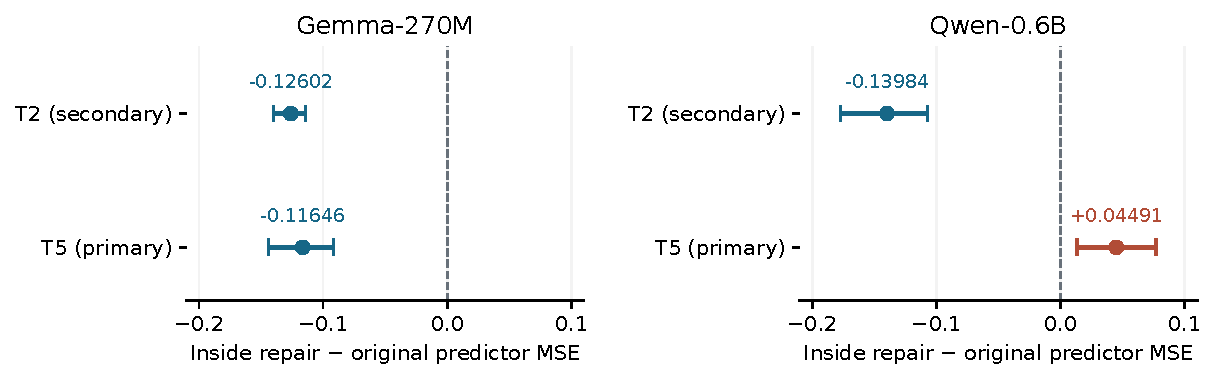
\includegraphics[width=.92\textwidth]{aligned_repair.pdf}
\caption{The sign of inside-space repair depends on the tested model/frame. Points and nominal pointwise 95\% intervals are copied from accepted block summaries, with no new resampling. Negative means lower error in the predicted intervention effect. Separate model panels avoid treating squared-logit magnitudes as a paired architecture ranking.}\label{fig:aligned}
\end{figure}
\subsection{Earlier held-out tests also establish harm}
Separate single-fit tests provide additional evidence that oracle inside-space repair need not help. On primary T5, Gemma-1B has mean loss change $+.50370$ (saved 99\% interval $[.43370,.57832]$, family-adjusted $p=.003$); Llama-1B has $+.77826$ ($[.66913,.89066]$, adjusted $p=.002$). Each uses 256 blocks with its own frozen fit and original decision family. Llama's secondary T2 effect is beneficial, $-.40679$ ($[-.47176,-.35053]$), and remains descriptive. These are separate held-out studies, not an equal-baseline architecture comparison or a combined four-model significance test.

Gemma also tests whether adding frame-specific vector responses improves transfer and induces a predicted vector/readout ranking reversal. The transfer contrast succeeds, but the ranking reversal does not: the space that removes more vector error also has lower readout loss on the fresh T5 cohort. Thus the three prespecified hypotheses do not jointly succeed. Appendix~\ref{sec:earlier} retains their definitions, full table and inference corrections. This failed prediction motivates the fitted-object diagnostic below; it is not discarded in favor of the successful harm contrast.
\section{Why a historical ranking does not transfer unchanged}
The failed Gemma ranking prediction prompted a posthoc crossed diagnostic. Here $U_2$ and $U_5$ are rank-eight spaces whose response-fitting samples were augmented with equal numbers of T2 and T5 documents, respectively; $P$ is held fixed when comparing them. We write $L(U_k)$ as shorthand for the loss after oracle repair using $U_k$. On identical cached T5 states and native targets, we exchanged historical/current $P$ and historical/current $U_2,U_5$ pairs. The complete displayed Gemma analysis uses the historical 32-block cohort and the current 256-block cohort, with all four conditions. Diagonal reproduction checks passed; no predictor was refitted and no new full-model run was required.

For both predictors and both cohorts, the mean sign of $L(P_{U_5})-L(P_{U_2})$ followed the subspace-pair version: positive with the historical pair and negative with the current pair. Table~\ref{tab:crossed} displays the complete current-cohort cross; the evidence retains both cohorts. This is a controlled substitution of fitted matrices on fixed states, not identification of a training-domain cause, a universal ordering, or a claim about every record.
\begin{table}[ht]\centering\small
\begin{tabular}{llr}\toprule Predictor & Subspace pair & Mean $L(U_5)-L(U_2)$\\\midrule
P old & old & 0.24262 \\
P old & new & -0.42739 \\
P new & old & 0.06128 \\
P new & new & -0.07894 \\
\bottomrule\end{tabular}
\caption{Gemma-1B posthoc T5 substitutions on the same 256-block cohort. No fresh confirmatory $p$-value is assigned.}\label{tab:crossed}
\end{table}

\section{Can a forecast guide a useful learned repair?}
\subsection{Separating oracle information from learned correction}

Let $r=D-P$, $c=UU^\top r$, and let $J$ be the analytic gradient of the actual final norm/two-head-row readout at the predicted state $P$. The frozen first-order score is
\[
 s=(Jc)^2-2(Jr)(Jc).
\]
It forecasts the sign of the \emph{finite} measured loss change; it is not an exact nonlinear identity. It uses true $D$ and native head/gradient information. After exploratory work, the forecast formula, ties and reporting were frozen before the subsequent finite head outcomes. Accuracy on these finite cohorts is not a population guarantee.

For a learned alternative, keep $P$ from FIT\_MAP fixed and fit an affine residual ridge $\widehat r(x_d-x)$ on the disjoint FIT\_U vector labels $D-P$, with the same scale/centering/$\lambda=.01$ recipe. $U_0$ also uses FIT\_U native responses; these two fitted objects are therefore not independent. The no-$D$ correction is $\widehat c=UU^\top\widehat r$, with score
\[
 \widehat s=(J\widehat c)^2-2(J\widehat r)(J\widehat c),
 \qquad P_{gate}=\begin{cases}P+\widehat c,&\widehat s<0,\\P,&\widehat s\geq0.\end{cases}
\]
Only the recipient residual $R$, branch input $x$, native branch output $y$, and the donor branch input enter the feature function; donor $y$/TEST $D$ and finite intervention readouts do not choose this correction or gate. Native captured records are deserialized, so the claim is about construction/use, not absence of truth arrays from disk. No-$D$ forecasts are immutably sealed before oracle reference construction and finite repair readouts. The method still needs native prefix states and readout-gradient access.

Report unconditional loss against $P$, always-applied projection, full $P+\widehat r$, and a strong direct ridge trained on the same available MAP$\cup$U 256 vector labels. The full residual score is $-(J\widehat r)^2\leq0$, so its gate is algebraically trivial apart from exact ties. Oracle and learned variants change \emph{both} correction vectors and scores; their accuracy gap does not isolate removal of $D$ from identical interventions.

\subsection{The aligned Qwen test: better signs do not ensure lower loss}

The new Qwen study also executes the fixed no-$D$ recipe. Table~\ref{tab:qgate} keeps strong alternatives visible rather than judging only sign accuracy.
\begin{table}[ht]\centering\small
\begin{tabular}{lrrrrr}\toprule
Frame & $P$ & Always proj. & Gate & Full residual & Direct256\\\midrule
T5 & 0.490827 & 0.566921 & 0.521107 & 0.444232 & 0.379464 \\
T2 & 0.672181 & 0.608098 & 0.594775 & 0.535158 & 0.505563 \\
\bottomrule\end{tabular}
\caption{New Qwen-0.6B unconditional losses on 256 blocks. All nine fitted crosses remain secondary.}\label{tab:qgate}
\end{table}

Oracle sign accuracy is 99.479\% on T5 and 99.837\% on T2. Learned sign accuracy is 64.746\% and 68.620\%, compared with 63.249\% and 59.375\% for the better constant sign rule. Coverage is 100\% with no ties. This gives descriptively better sign accuracy than the constant rule in this Qwen scope; it does not overturn the supporting scopes, where the learned sign rule loses to that baseline. Yet the gate still harms relative to $P$ on primary T5, and pooled direct256 is better on both frames. The gate beats the always-projected policy on both frames; on T2 it also beats never applying repair. Sign prediction, oracle repairability and useful correction remain distinct estimands. These dependent-cell accuracy fractions are descriptive, not population binomial certifications.

\subsection{Supporting evidence from three other study scopes}
The earlier 32-block uniform-$U_0$ study provides a separate check on the forecast/utility distinction, using three matched fits on Gemma-1B, Llama-1B and Gemma-270M. Oracle sign accuracies are 99.22\%, 99.74\% and 99.48\%, respectively, including scopes where oracle repair itself is harmful. Learned sign accuracies are 39.84\%, 65.62\% and 58.07\%, versus 60.94\%, 72.40\% and 62.50\% for the better constant sign rule. All three learned accuracies are lower than that baseline. In all three rows, the learned gate is worse than the better of always applying the learned projection or never applying it. The full loss table and timing qualifications are in Appendix~\ref{sec:c3}. These small-cohort results support the distinction; they do not enlarge the aligned 256-block sample.
\section{Discussion and conclusion}
The fresh L21 studies identify a prediction-error component that is highly oracle-correctable in the tested setting, then demonstrate learned usefulness on separate fresh data. The unchanged historical rank-eight space supports a 99.25\% oracle readout-MSE reduction; a learned coefficient correction supports a 97.21\% reduction relative to the historical predictor on another 64 blocks. These are different cohorts and interventions on prediction error, not an equality between oracle and learned performance. The space was fitted from native vector responses without direct readout labels. Separate rank/norm controls favor FIT-derived spaces over the fixed random draws; ranks 16 and 32 improve further, so neither an intrinsic dimension eight nor optimality is established.

The baseline comparison is decisive for interpretation. Direct384 has lower mean loss than learned correction despite using the same additional 384 vector labels, and a linear direct predictor restricted to $U$ also has slightly lower point loss. A constant mean correction worsens the historical predictor. The fresh budget TEST additionally identifies a conditional C32 advantage of 48.03\% over Direct32, but Direct has lower mean loss at 64--384 labels (the 256/384 contrast intervals include zero) and C64 worsens relative to C32. Three new FIT32 cohorts on the reused TEST favor Direct on average for have/has; the is/are mean interval includes zero. The C32 advantage belongs to one fixed training sequence; two of the later is/are fits have negative point contrasts, but the mixed three-fit result does not establish stable superiority. Thus the evidence supports scoped learned utility and an observed conditional advantage. C is prior-centered kernel ridge, with an exact linear prior interpretation under the conditions in Section~\ref{sec:priorridge}; it is not a new or inherently more expressive regression algorithm. Historical training information is not equalized by matching the additional label count. Native prefix computation is still needed.

The L27/L17 and earlier tests establish limits rather than contradicting this L21 result. The same three Qwen L27 fitted pairs help on T2 and harm on T5; Gemma-270M benefits on both, while separate Gemma-1B and Llama-1B cohorts establish T5 harm; Llama benefits on T2. Their operators, layers and fitting recipes differ, preventing a causal attribution to layer alone. In L27, accurate oracle sign forecasts coexist with a gate that worsens Qwen T5, and Direct256 has lower mean loss on both frames. Repairability, learned utility and advantage over direct prediction therefore remain distinct empirical questions.

Most conclusions concern one is/are margin in synthetic contexts; the posthoc have/has extension tests another grammatical margin on the same prompts, selected checkpoints/operators and fixed fits. Fresh pairs do not undo historical selection of the favorable L21 regime. Nominal intervals do not establish fit-population stability or familywise claims; fixed random controls do not sample the entire distribution of possible spaces. The empirical contribution is the controlled sequence from oracle-correctable error to measured learned utility and its limits, with negative baseline comparisons retained. Public release still requires complete authorship, evidence availability and campaign disclosures.


\appendix
\section{Detailed designs and fitting}
\label{sec:methods}

\subsection{Models and fitting}
The earlier single-fit tests use local Gemma-3-1B-pt and Llama-3.2-1B checkpoints. Native capture and branch evaluation use FP32; regression and subspace arithmetic use FP64. The final transformer block and final prompt position are tested. Gemma includes its post-feedforward branch normalization; Llama uses its raw MLP output. The recipient residual remains fixed. The actual final norm and output head, including configured softcaps, determine the readout. Exact-prefix/branch checks and native parity were qualified before the respective tests.

Each model has its own predictor and subspace. FIT\_MAP and FIT\_U each contain 128 documents: 16 distinct lexical blocks, two fitting frames and four subject/distractor conditions per block. With input differences $X$, use one global scale $s=\sqrt{\operatorname{mean}(X^2)}$, $Z=X/s$, and centered ridge regression with an unpenalized intercept:
\[
 A=Z-\bar Z,\ B=D-\bar D,\quad W=A^\top(AA^\top+n\lambda I)^{-1}B,
 \quad P=ZW+\bar D-\bar ZW,\quad\lambda=.01.
\]
$U_0$ is the leading eight right singular vectors of the uncentered FIT\_U response matrix. The Llama implementation stores the dense map and implements this centered ridge equation. No TEST labels are used to fit these objects.

\subsection{Frames and units}
Each TEST contains 256 lexical blocks, with four subject-side/distractor conditions within each frame. Gemma measures T0, T2, T5, T6 and T7, yielding 5120 recipient documents. Llama's reduced replication measures T2 and T5, yielding 2048 documents. Its removal of additional arms limits diagnosis; it preserves the basic $P/U_0$ contrast and fitting recipe. Blocks, not individual condition rows, are the resampling units. Both results condition on one model-specific frozen fit.

T2 uses ``Near the enclosure, the \{s\} that the \{a\} can observe''. T5 uses ``Everyone agrees that the \{s\}, unlike the \{a\},''. T6 changes the surrounding context/preposition; T7 adds a parenthetical construction. Donors reverse subject number within the same block, frame and distractor condition. The readout is logit(` is') minus logit(` are'), including leading spaces in tokenizer queries. Lexical freshness refers to the recorded local exposure audit, not pretraining.

\subsection{Gemma's additional contrasts}
$U_2$ and $U_5$ augment the original response fit with 64 vector-response documents of T2 and T5, respectively. $U_{ctrl}$ adds the same number from fitting-style T0 on the same additional lexical blocks. Rank and $P$ remain fixed. This controls sample count and added vocabulary, but does not isolate exact-frame coverage from every possible kind of off-fit diversity.

Three hypotheses were fixed before the new TEST. A1 asks whether $U_2$ reduces readout loss relative to $U_{ctrl}$ on the equal-weight T6/T7 mixture. A2 requires both lower vector error for $U_5$ than $U_2$ on T5 and higher readout loss for $U_5$. A3 asks whether original-$U_0$ repair harms relative to $P$ on T5. A2 is a conjunction, not a result established by its vector component alone.

The historical observations motivated these predictions; fresh tests do not retroactively make those observations prospective. An initially proposed joint-power gate was infeasible. A prospective fixed-$N=256$ amendment removed the 80\% power assurance, while retaining the scientific hypotheses and analysis. Statistical calibration and acquisition acceptance are separate receipts. No test outcome was used to change these hypotheses, fit, sample size or frames.

\subsection{Distinct stages, not a cumulative replication count}
The earlier single-fit Gemma/Llama tests retain their original decision families. The 32-block three-fit forecast study combines prospective Llama/Gemma-270M acquisition with a retrospective Gemma-1B extension. The aligned 256-block Gemma-270M/Qwen studies share lexical blocks but not model measurements, and use L17/L27, unlike the fresh L21 experiments. The oracle and learned384 L21 TEST cohorts each contain 64 different pairs. The budget test adds a third 64-block cohort; the subsequent new-FIT/readout test reuses that budget TEST posthoc. The 24 historical FIT blocks are reused, and the latter test adds six new FIT blocks. None of these cohorts or fixed fitted objects can be added as independent replications of one claim. Checkpoint and full source identities remain in the evidence manifest.

\section{Earlier confirmatory tests and failed ranking prediction}
\label{sec:earlier}

\subsection{Gemma: harm and transfer, but no ranking reversal}
Table~\ref{tab:gemma} reports the fixed Gemma family. Positive A1 means a benefit from $U_2$ relative to the count control. Positive A3 means harm from $U_0$ relative to $P$. The component intervals are saved pointwise 99\% intervals, not simultaneous intervals for all rows.
\begin{table}[ht]
\centering\small
\begin{tabular}{lrrr}
\toprule Contrast & Estimate & 99\% interval & Family-adjusted $p$\\
\midrule
A1: $L(U_{ctrl})-L(U_2)$ & .09175 & [.06919,.11690] & .003\\
A2 vector: $V(U_2)-V(U_5)$ & 89573.33 & [82967.58,95928.14] & ---\\
A2 readout: $L(U_5)-L(U_2)$ & -.07894 & [-.12404,-.03467] & 1.000\\
A3: $L(U_0)-L(P)$ & .50370 & [.43370,.57832] & .003\\
\bottomrule
\end{tabular}
\caption{Gemma, 256 blocks. Readout units are squared logits; vector units differ. A2's displayed adjusted value is for its conjunction, not a separate vector test.}\label{tab:gemma}
\end{table}

A1 and A3 meet their prescribed criteria. A2 does not: although $U_5$ removes more vector error, its readout loss is lower, not higher, than $U_2$ on the new T5 cohort. The formerly observed opposite ranking is therefore not reproduced by this fresh test. The three hypotheses do not jointly succeed.

A retrospective cache audit compared historical selected T5 values $L(U_2)=.34412$ and $L(U_5)=.54561$ with new values $.23150$ and $.15256$. New lexical data and fitted objects differ. This diagnoses a change in the empirical ranking; it does not isolate the causal contribution of the fitting sample versus the test domain.

\subsection{Llama: primary harm and secondary benefit}
On the prespecified T5 contrast, Llama gives
\[
 \operatorname{mean}[L(U_0)-L(P)]=0.77826,
 \qquad 99\%\ \mathrm{CI}=[0.66913,0.89066].
\]
The fixed multiplicity-adjusted $p$ is .002. Thus the new Llama test supports harmful repair in the prescribed direction. The T2 secondary contrast instead gives $-.40679$, with saved 99\% interval $[-.47176,-.35053]$. It remains descriptive; it is not promoted to a new primary success.

These two frames show why the conclusion must be conditional. A repair constructed by the same recipe can harm in one context and benefit in another. The different Gemma and Llama effect magnitudes are not a paired causal comparison of architectures or an equal-baseline performance ranking.

\section{Supporting 32-block forecast and correction study}
\label{sec:c3}

Table~\ref{tab:c3} shows the permitted model scopes of the uniform-$U_0$ correction study. Each row averages three matched pairs and four conditions within 32 blocks (384 dependent cells). All nine pairwise crosses remain in the per-model evidence. These are not the latest 256-block experiments.
\begin{table}[ht]\centering\scriptsize
\resizebox{\textwidth}{!}{\begin{tabular}{lrrrrrr}\toprule
Model & $P$ & Oracle & Always proj. & Learned gate & Direct256 & Sign accuracy oracle / learned / constant\\\midrule
Gemma3-1B & 0.28114 & 0.81690 & 0.33862 & 0.32464 & 0.35122 & 99.22\% / 39.84\% / 60.94\% \\
Llama3.2-1B & 1.79614 & 3.05097 & 1.29969 & 1.33213 & 1.61029 & 99.74\% / 65.62\% / 72.40\% \\
Gemma3-270M & 0.41963 & 0.27832 & 0.34473 & 0.35505 & 0.37179 & 99.48\% / 58.07\% / 62.50\% \\
\bottomrule\end{tabular}}
\caption{Selected uniform-$U_0$ study; Losses are in squared-logit units; cross-model scales are not a controlled architecture ranking. Gemma-1B is retrospective; Llama/Gemma-270M native responses are prospective.}\label{tab:c3}
\end{table}

Oracle forecast accuracy is high even when the oracle repair itself is harmful (notably Llama). Learned projection helps relative to $P$ in Llama/Gemma-270M but harms in this Gemma-1B cohort. In all three displayed cases, the gate is worse than the better of always applying the projection or never applying it. Thus prediction accuracy with oracle information does not establish a useful learned policy. The three displayed scopes are selected from a broader program; this draft does not claim complete public campaign reporting.

\section{Inference, qualification and operation accounting}

The earlier single-fit Gemma/Llama decision families use 1999 paired block draws, recorded seeds and a finite Monte Carlo correction. The newer nominal/descriptive analyses do not inherit their p-value transforms or rejection claims. The earlier fixed analyses apply the frozen conservative transform $p_{safe}=\min(1,2p_{raw})$ before the respective family correction. Gemma applies Holm across its three hypotheses; the A2 conjunction retains both components. Llama uses the prospectively fixed two-slot replication correction, $\min(1,2p_{safe})$; that multiplier remains unchanged in this selected two-model manuscript. These are distinct families, so .003 and .002 must not be interpreted as a newly combined cross-model test. The intervals describe the fixed-fit block distribution and do not estimate uncertainty from independently refitting $P$ and $U$.

The acquisition and numerical analyses received separate independent checks. Gemma's sealed TEST contains 35,840 forward operations; Llama TEST contains 8192. They include full captures and cheaper branch/suffix operations, and are not equivalent-cost full-model passes. Existing valid cache was preserved during recovery. No model calls or resampling were performed to write this manuscript.

A separate repeated-fit stability qualification did not meet its global calibration gate. It supplies no positive stability finding and does not invalidate the conditional single-fit measurements. We do not claim 15 independent fitting replications, broad calibration for every population, or guaranteed power. Saved legacy status strings in copied evidence describe their original computation stage; the subsequent approved acquisition receipt is supplied as \path{evidence/review_errata/gemma_acquisition_review.json}, with its bound completion snapshot. It supersedes the pending acquisition wording without altering the preserved historical records.

The aligned Gemma extension used 2048 full captures and 20480 cheaper final-norm/head operations (22528 heterogeneous forwards, zero backward, one full-model load), reusing three accepted fits and technical qualification. Qwen used 2844 capture/control operations and 102400 head operations (105244 heterogeneous forwards, zero backward, one full-model load), plus 6144 unique analytic-gradient points evaluated 18432 times during deterministic regeneration. A schema-only first head attempt failed before any FIT/head call and consumed zero scientific operations; its records remain preserved. Coupled immutable receipts retain every logical operation despite using fewer filesystem objects. These counts are not equal-cost full-transformer passes. The new analyses received independent source/data/accounting/output reviews. The L21 extension separately used 35 technical qualification forwards and 66,284 logical MAIN forwards, with 372 identical-target aliases covering all 66,656 scheduled slots, zero backward operations and one model load per stage. MAIN comprises 1,024 conditions; aliases avoid duplicate evaluations. Independent review verified all 62 arm MSEs and block means, all 9,789 sealed files, accounting and norm matching. Full-vs-batched suffix parity was qualified at maximum absolute margin difference $1.05\times10^{-5}$ against the frozen $10^{-4}$ tolerance. No model calls, refits or resampling were performed to prepare this manuscript.


The learned L21 stage reuses 384 FIT labels without new training acquisition. Its prospective stage uses 8,460 logical forwards in 3,336 physical calls (zero backward, one load), including 12 full/suffix FIT qualification calls. All 256 natural captures and 1,024 target-free prefixes precede the global prediction freeze; 1,024 native targets and six-arm batched suffix evaluation follow. Qualification error is at most $3.82\times10^{-6}$ at the frozen $10^{-4}$ tolerance. Independent completion review reconstructs all 1,024 rows and checks freeze order, saved targets, aggregates and accounting. No model evaluation or bootstrap is repeated for the manuscript.

\section{Evidence and reproducibility}
The accompanying evidence directory preserves Gemma's original primary result, its source manifest and independent numerical review, and Llama's final result and independent review. Local canonical acquisition receipts bind the complete raw caches and model-specific fits. Manuscript tables reproduce saved summaries without recomputing inference. Model weights are not distributed in this source bundle. Repeating native measurements requires the recorded checkpoint identities, tokenization and hook configurations, frozen protocols and environment.

All earlier drafts remain preserved separately. This fourteenth draft integrates the independently accepted fresh L21 oracle/rank, learned384, budget and three-new-FIT/readout studies and the November 4 editorial and algebraic corrections into the repair question while preserving all earlier single-fit decision families and negative findings. The evidence includes the L21 summary, protocol and numerical amendment, completion audit/review, full hash-binding snapshot, and the preserved selected earlier per-model summaries; no native measurements, fits or resampling were repeated to write it. Only Gemma-270M and Qwen-0.6B have the aligned 256-block inside/outside comparison; the oracle, learned384 and budget L21 TEST studies have separate cohorts; the subsequent new-FIT/readout test reuses the budget cohort posthoc. The 32-block correction data and earlier single-fit 256-block tests remain separate. It is not a public preprint submission. Author names, affiliations, public release location, model-license disclosures and AI-assistance statements require human completion before submission.
\clearpage
\section{All matched fits in the new aligned study}\label{sec:perfit}
\begin{table}[ht]\centering\scriptsize
\resizebox{\textwidth}{!}{\begin{tabular}{llrrrrrr}\toprule
Model & Fit & T5 $P$ & T5 inside & T5 outside & T2 $P$ & T2 inside & T2 outside\\\midrule
Gemma-270M & r1 & 0.349194 & 0.314874 & 0.061504 & 0.220346 & 0.091935 & 0.049198 \\
Gemma-270M & r2 & 0.356221 & 0.188821 & 0.196827 & 0.219166 & 0.068236 & 0.082416 \\
Gemma-270M & r3 & 0.641876 & 0.494210 & 0.234445 & 0.188325 & 0.089597 & 0.036322 \\
Qwen-0.6B & r1 & 0.410719 & 0.487814 & 0.121515 & 0.708276 & 0.544488 & 0.065037 \\
Qwen-0.6B & r2 & 0.744981 & 0.756218 & 0.076390 & 0.688982 & 0.574276 & 0.057373 \\
Qwen-0.6B & r3 & 0.316781 & 0.363163 & 0.127169 & 0.619285 & 0.478255 & 0.076956 \\
\bottomrule\end{tabular}}
\caption{Saved per-fit point estimates; no per-fit significance family or fit-population inference is added.}\end{table}

\small
